%%%%%%%%%%%%%%%%%%%%%%%%%%%%%
%  MODELO (TEMPLATE)
%  Comandos e funções para utilização deste Modelo (Template)
%%%%%%%%%%%%%%%%%%%%%%%%%%%%%
\chapter*{Modelo ({\it template}) COEEL:  Utilizando a classe~``cls-PFC-COEEL.cls''}

Modelo (Template) ~\LaTeX ~da classe: {\bf cls-PFC-COEEL.cls} criada pelo professor Elvio, para atender às demandas de \textbf{PFC - Projeto de Fim de Curso} de Engenharia Elétrica (\gls{COEEL}) do IFBA {\it campus} Vitória da Conquista e \textbf{Relatórios Técnicos} de disciplinas.

{\bf Para a utilização deste Modelo ({\it template}) você precisará possuir conhecimento básico de programação em ~\LaTeX}. Caso você esteja entrando em contato com~\LaTeX~ pela primeira vez, recomendo que procure um minicurso básico ou estude vídeos de introdução ao~\LaTeX~no Youtube. Não trataremos de comandos básicos de ~\LaTeX~ neste modelo.

Este modelo foi criado e testado no  {\bf \LaTeX-Overleaf} para ser compilado em {\bf pdfLaTeX} ou {\bf XeLaTeX}.

Segue uma dica importante com o comando \verb|\begin{CaixaVermelha}|:

\begin{CaixaVermelha}
    {\bf Dica:} Membros do {\bf \gls{IEEE}} com membresias ativas de estudantes ou professores, possuem acesso total ao Overleaf com todas as funções desbloqueadas.
\end{CaixaVermelha}

Agora a mesma dica com o comando \verb|\begin{CaixaVerde}|:

\begin{CaixaVerde}
    {\bf Dica:} Membros do {\bf \gls{IEEE}} com membresias ativas de estudantes ou professores, possuem acesso total ao Overleaf com todas as funções desbloqueadas.
\end{CaixaVerde}

Neste capítulo você encontrará a forma na qual este Modelo ({\it template}) foi organizado e dicas de como utilizar os comandos específicos criados para a classe \verb|cls-PFC-COEEL.cls|~ de forma a atender às demandas da COEEL. 

%%%%%%%%%%%%%%%%%%%%%%%%%%%%%
\pagebreak\newpage\clearpage

\section{Organização do Modelo ({\it template}) - \LaTeX -Overleaf}

A organização do Modelo ({\it template}) no ~\LaTeX -Overleaf, segue conforme mostra a figura~\ref{fig:Organiza_Template}.

 \begin{figure}[htb]
     \centering
     \FonteFig{Próprio Autor}
     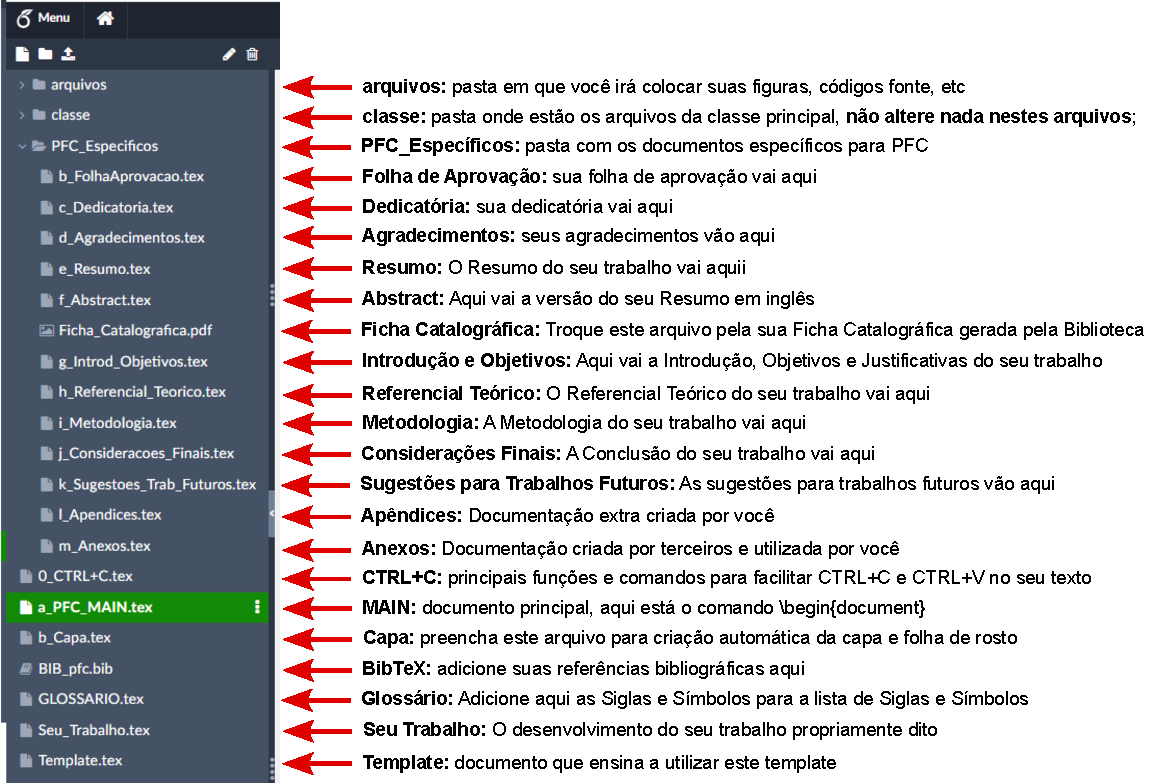
\includegraphics[width=14cm]{classe/arqcls/Organiza_template.pdf}
     \caption{Organização deste Modelo ({\it template}) no Overleaf}
     \label{fig:Organiza_Template}
 \end{figure}

\begin{CaixaVermelha}
    \begin{enumerate}
        \item {\bf IMPORTANTE:}  Não alterar nenhum documento dentro da pasta {\bf classe}. Os arquivos desta pasta possuem os comandos de formatação deste {\it template} que foi aprovado pelo colegiado da coordenação COEEL, logo não é permitido nenhuma alteração;
        \item O conteúdo da pasta {\bf arquivos} pode ser alterado e modificado livremente;
        \item O conteúdo da pasta {\bf arqcls} são as figuras e códigos exemplo deste modelo ({\it template});
        \item a pasta {\bf PFC\_Especificos} contém os documentos específicos e exclusivos para PFC e foram organizados nesta pasta;
        \item o documento {\bf 0\_CTL+C.tex} contém as funções mais utilizadas, de fácil acesso, para você utilizar CTRL+C e CTRL+V.
    \end{enumerate}
\end{CaixaVermelha}
 

%%%%%%%%%%%%%%%%%%%%%%%%%%%%%

\section{Selecionar a classe para o modo de PFC ou modo de Relatório}

Este Modelo ({\it template}) pode ser utilizado para a produção de Monografias de {\bf PFC (Projeto Final de Curso)} de Egenharia Elétrica, e também para {\bf Relatórios} de disciplinas.

Para habilitar este modelo para funcionar como {\bf PFC}, altere o documento principal (Main) conforme mostra o código~\ref{cod:PFC}: 

\ImportaCodigo[language=tex, caption=Para produzir PFC-Projeto Final de Curso, label=cod:PFC]{classe/arqcls/Cod_PFC.txt}

Para habilitar este modelo para funcionar como {\bf Relatório de Disciplina}, altere o documento principal (Main) conforme mostra o código~\ref{cod:Relat}: 

\ImportaCodigo[language=tex, caption=Para produzir Relatório de Disciplina, label=cod:Relat]{classe/arqcls/Cod_Relat.txt}

%%%%%%%%%%%%%%%%%%%%%%%%%%%%%
\pagebreak\clearpage\newpage

\section{O que deve ser preenchido para a geração automática da parte Pré-Textual do seu trabalho}

{\bf Para gerar automaticamente a Capa e Folha de Rosto:} Entre no documento principal (\verb|a_PFC_main.tex|), e procure pelos comandos listados abaixo, perceba que existem locais apropriados para preenchimento caso seja um PFC ou Relatório:

\begin{itemize}
    \item {\Large \verb|\Titulo{}|:} adicionar o título do seu trabalho aqui;
    \item {\Large \verb|\Autor{}|:} preencha com o seu nome;
    \item {\Large \verb|\Professor{}|:} preencha somente se for Relatório;
    \item {\Large \verb|\Disciplina{}|:} preencha somente se for Relatório;
    \item {\Large \verb|\Orientador{}|:} preencha somente se for PFC;
    \item {\Large \verb|\Coorieantador{}|:} preencha somente se for PFC;
    \item {\Large \verb|\DataDefesa{}|:} preencha com a data de defesa do PFC ou com a data de entrega do relatório, caso não saiba a data, deixe \verb|\today|;
    \item {\Large \verb|\CidadeDefesa{}|:} a cidade sempre será Vitória da Conquista, pois trata-se da cidade onde se encontra a COEEL;
\end{itemize}

%%%%%%%%%%%%%%%%%%%%%%%%%%%%%
\pagebreak\clearpage\newpage

\section{Procedimentos da Biblioteca para solicitação da Ficha Catalográfica}
\label{sec:Biblioteca}

A ficha catalográfica é um serviço prestado pela Biblioteca. 

Para confecção de Ficha Catalográfica, o bibliotecário segue as regras e normas
internacionais do Código de Catalogação Anglo-Americano - 2ª edição (AACR2).

{\bf PROCEDIMENTO:}

A solicitação deverá ser feita quando o aluno já tiver apresentado seu trabalho para a Banca Examinadora e feito todas as correções sugeridas.

As palavras-chave devem ser de três a cinco. Devem ser palavras que identifiquem o tema do trabalho que, isoladas, proporcionem ao leitor o entendimento do assunto do trabalho.

{\bf PARA ONDE ENVIAR A SOLICITAÇÃO:}

A solicitação para elaboração da ficha deverá ser feita exclusivamente por meio do e-mail da Biblioteca- \url{biblio.ifba.conquista@gmail.com}

{\bf PRAZO DE RESPOSTA:}

O prazo de resposta das solicitações (de ficha ou alteração de fichas já enviadas) é de até 06 (seis) dias "úteis" a depender da demanda do serviço. Por isso, recomendamos que não deixe seu pedido para a última hora, pois a demanda é alta em períodos de entrega da versão final.

Fiz o meu pedido há mais de 6 dias e não tive respostas. O que fazer? Neste caso, entre em contato com a Biblioteca, pois pode ter tido algum problema no recebimento do e-mail.

{\bf OUTRAS INFORMAÇÕES:}

Os usuários com pendência na Biblioteca não poderão solicitar o serviço;

A ficha catalográfica deverá estar localizada na parte inferior do verso da folha de rosto, de forma centralizada no trabalho impresso e também deve constar no trabalho em formato digital;

A ficha catalográfica deve ser anexada na íntegra, ou seja, não é permitido ``recortar'' ou omitir informações disponíveis no documento, e não deve ser alterada sem permissão do bibliotecário;

As fichas catalográficas são enviadas no formato de arquivo não editável para garantir a formatação da peça. Se o solicitante identificar erros de digitação ou de inserção de
dados pode solicitar a biblioteca a correção dos erros;

A ficha catalográfica deverá ser inserida na parte inferior do verso da Folha de Rosto do trabalho. A folha da ficha catalográfica deve ser contada para a paginação, mas não numerada, por ser um elemento pré-textual.

De acordo com a Resolução n. 184, de 29 de setembro de 2017, do Conselho
Federal de Biblioteconomia (CFB), a ficha catalográfica deve estar acompanhada do
nome e do número de registro profissional do bibliotecário que a elaborou. Portanto,
solicitamos que as informações da ficha não sejam alteradas. Se necessitar de qualquer alteração na ficha, por favor, solicite-a a bibliotecária.

%%%%%%%%%%%%%%%%%%%%%%%%%%%%

\subsection{Como adicionar automaticamente o PDF da Ficha Catalográfica}

Após sua defesa do PFC perante a banca avaliadora, caso seu trabalho tenha sido aprovado, você realizará as correções sugeridas pela banca e pelo seu orientador.

Após aprovação do texto você precisará solicitar a Ficha Catalográfica para a Biblioteca do campus, conforme orientações da seção~\ref{sec:Biblioteca} da página~\pageref{sec:Biblioteca}.

Para acrescentar automaticamente o PDF da Ficha Catalográfica fornecida pela Biblioteca no seu documento, abra o documento principal {\bf a\_PFC\_main.tex} e procure pela parte que trata sobre a Ficha Catalográfica, como mostra o código~\ref{cod:FichaCatalografica} a seguir.

Faça upload do PDF da sua Ficha Catalográfica no ~\LaTeX~Overleaf~ e substitua o arquivo PDF chamado: \verb|Ficha_Catalografica.pdf| pela sua Ficha Catalográfica, e caso o nome do PDF seja diferente, renomeie o nome do PDF no código~\ref{cod:FichaCatalografica}. Desta forma o ~\LaTeX~ irá importar e adicionar sua Ficha Catalográfica automaticamente no seu documento.

\pagebreak

\begin{Codigo}[language=tex, caption=Código da Ficha Catalográfica no documento principal {\bf a\_PFC\_main.tex}, label=cod:FichaCatalografica]
    %%%%%%%%%%%%%%%%%%%%%%%%%%%%
    %%%% FICHA CATALOGRAFICA
    % apenas para PFC
    %
    \ifbool{pfc}{ 
        \newpage\clearpage\pagebreak
        \ifpdf\phantomsection\fi
        \addcontentsline{toc}{chapter}{Ficha Catalografica}
        % inclua o PDF da ficha catalografica 
        % feita pela biblioteca
        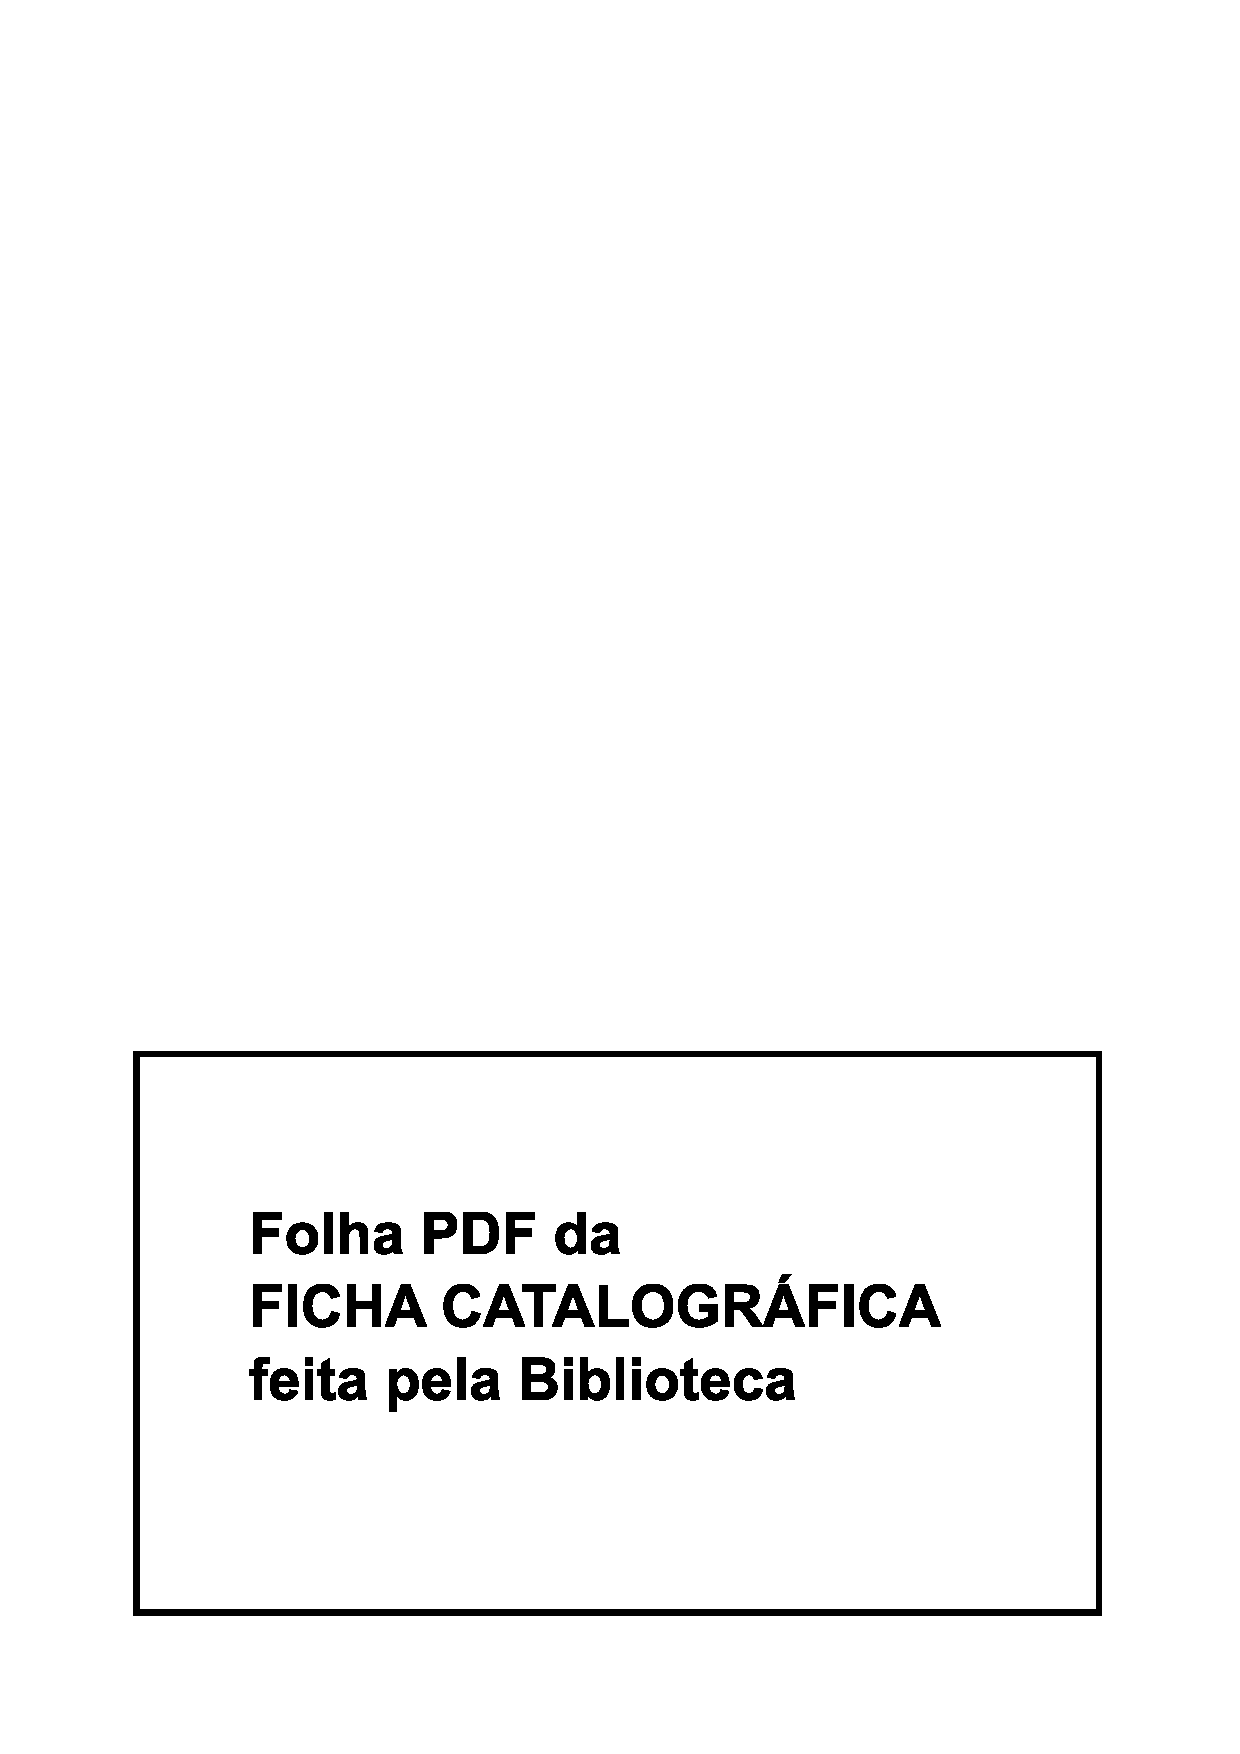
\includepdf[pages=1]{Ficha_Catalografica.pdf}
    }{}
\end{Codigo}

%%%%%%%%%%%%%%%%%%%%%%%%%%%%%%

\section{Adicionando automaticamente o PDF da Folha de Aprovação}

Verifique o documento chamado \verb|b_FolhaAprovacao.tex|. 

Caso a Folha de Aprovação de seu trabalho precise ser assinada manualmente, à caneta, preencha o nome, titulação e campus dos membros da banca, imprima esta folha PDF e a leve no dia de sua defesa para que a banca possa assiná-la à caneta, depois você irá escaneá-la e adicioná-la da mesma forma que se adiciona a Folha de Aprovação assinada digitalmente, no documento principal \verb|a_PFC_main.tex|, conforme mostra o código~\ref{cod:FolhaAprovacao}.

Caso a Folha de Aprovação de seja assinada digitalmente pelo sistema SEI ou pelo SOU.GOV, seu orientador irá providenciar a confecção da Folha de Aprovação e providenciará a assinatura dos membros da banca e você irá adicioná-la ao seu trabalho, no documento \verb|a_PFC_main.tex| da conforme mostra o código~\ref{cod:FolhaAprovacao}. Renomeie o PDF da sua Folha de Aprovação assinada para \verb|Folha_Aprovacao.pdf| e faça o upload do PDF para o ~\LaTeX~Overleaf. 

\pagebreak

\begin{Codigo}[language=tex, caption=Código da Folha de Aprovação no documento principal {\bf a\_PFC\_main.tex}, label=cod:FolhaAprovacao]
    %%%%%%%%%%%%%%%%%%%%%%%%%%%%
    %%%% FOLHA DE APROVACAO
    % Apenas para PFC
    %
    \ifbool{pfc}{ 
        \newpage\clearpage
        \ifpdf\phantomsection\fi
        \addcontentsline{toc}{chapter}{Folha de Aprovacao}
    
        \includepdf[pages=1]{Folha_Aprovacao.pdf} 

        % comente esta linha quando 
        % for anexar o PDF
        % %%%%%%%%%%%%%%%%%%%%%%%%%%%%%%%%%%%%%%%%%%%%%
%%%%%% FOLHA DE APROVAÇÃO
%%%%%%%%%%%%%%%%%%%%%%%%%%%%%%%%%%%%%%%%%%%%%

% caso queira incluir o PDF da folha de aprovação assinada digitalmente pelos membros da banca pelo SEI ou pelo SOU.GOV, acrescente o arquivo PDF utilizando o comando seguinte comando dentro do arquivo MAIN:
% \includepdf[pages=1]{Folha_Aprovacao.pdf} % descomente esta linha se for anexar o PDF

  \clearpage\newpage\pagebreak%
  \pagestyle{plain}
  \begin{center}%
    \textbf{\Large \@Titulo  }\\%
    \vspace{1.2cm}%
    \MakeUppercase{\textbf{\Large \@Autor}}\\%
  \end{center}%
  \vspace{0.6cm}%

  A presente Monografia, apresentada em sessão realizada em \textbf{ \@DataDefesa}, foi avaliada como adequada para a obtenção do Grau de Bacharel em Sistemas de Informação, julgada \textbf{aprovada} em sua forma final pela Coordenação do Curso de Sistemas de Informação do Instituto Federal de Educação, Ciência e Tecnologia da Bahia, \textit{campus} Vitória da Conquista.

  \begin{center}
    
    \vspace{7mm}
    Vitória da Conquista/BA, \@DataDefesa.
    \vspace{7mm}
    \vspace{7mm}
    \rule[0cm]{10cm}{0,5mm}\\
    \textbf{}
    Prof. Me. Alexandro dos Aantos Silva\\
    (Coordenador do Curso - IFBA campus Vitória da Conquista)\\
    \vspace{7mm}
    \textbf{\small BANCA EXAMINADORA:}\par
    \vspace{7mm}
    \rule[0cm]{10cm}{0,5mm}\\
    Prof. DSc. Djan Almeida Santos (Orientador)\\
    IFBA campus Vitória da Conquista\\
    \vspace{7mm}
    \rule[0cm]{10cm}{0,5mm}\\
    Prof. Msc. Crijina Chagas Flores\\
    IFBA campus Vitória da Conquista\\

    \vspace{7mm}
    \rule[0cm]{10cm}{0,5mm}\\
    Prof. Msc. Liojes de Oliveira Carneiro\\
    IFBA campus Vitória da Conquista\\
    
  \end{center}
  
  
  % \vfill % leva para o botton da página
  % \begin{center}%    
  %   {\large  \@CidadeDefesa}\\%
  %   \vspace{1mm}%
  %   {\large  \@DataDefesa }%
  % \end{center}%
 
    }{}
\end{Codigo}

%%%%%%%%%%%%%%%%%%%%%%%%%%%%%

\section{Glossário: Comando ``gls'' para  gerar automaticamente lista de Símbolos e Siglas}
\label{sec:Glossario}

Verifique que existe um documento chamado: \verb|g_Glossario.tex|, abra este documento e verifique que este documento é uma Biblioteca de Lista de Siglas e Símbolos. Preencher este documento com as Siglas e com os Símbolos utilizados no seu documento.

Abra e veja o código~\ref{cod:Glo1}, você irá preencher o {\bf apelido} com um apelido para a sigla ou símbolo que será citado; preencher o {\bf name} com o nome da sigla ou símbolo que irá aparecer no texto; preencher o {\bf description} com a descrição do que é a sigla ou símbolo. Note que em alguns casos o {\bf apelido} e o {\bf name} poderão ser iguais.

\pagebreak

\begin{Codigo}[language=tex, caption=Biblioteca de Glossários~ {\bf g\_Glossario.gls}, label=cod:Glo1]
   \newglossaryentry{apelido} 
    {
    name = {Nome que aparece no texto},
    description = {Descricao da sigla ou simbolo}
    }
\end{Codigo}

Vamos dar um exemplo de como preencher o \verb|g_Glossario.tex| e como citar no texto as siglas e símbolos. Supondo que queremos colocar no glossário a sigla IEEE e que sua descrição seja: IEEE - Instituto de Engenheiros Eletricistas e Eletrônicos (IEEE is the world's largest technical professional organization dedicated to advancing technology for the benefit of humanity) e queremos citar a sigla $cos(\varphi)$ com descrição de {Fator de Potência} podemos adicionar o seguinte código no documento \verb|g_Glossario.gls|, como mostra o código~\ref{cod:Glo2}:

\begin{Codigo}[language=tex, caption=Biblioteca de Glossários~ {\bf g\_Glossario.gls}, label=cod:Glo2]
    % para SIGLAS
    \newglossaryentry{IEEE} % 
    {
    name = {IEEE},
    description = {IEEE - Instituto de Engenheiros
    Eletricistas e Eletronicos (IEEE is the world's 
    largest technical professional organization 
    dedicated to advancing technology for the benefit 
    of humanity)}
    }
    % para SIMBOLOS
    \newglossaryentry{FP}
    {
    name = {$cos(\varphi)$},
    description = {Fator de Potencia}
    }
\end{Codigo}

\begin{CaixaVermelha}
    Para que as siglas e símbolos apareçam no glossário, obrigatoriamente elas deverão ser citadas no texto.
\end{CaixaVermelha}

Para citarmos no texto as siglas e símbolos que adicionamos no documento \verb|g_Glossario.gls|, precisamos utilizar o comando \verb|\gls{}|, como por exemplo estou citando o \gls{IEEE} com o comando \verb|\gls{IEEE}| e o símbolo \gls{FP} com o comando \verb|\gls{FP}| no meu texto e automaticamente eles aparecerão no glossário. 

Note que as citações \gls{IEEE} e \gls{FP} aparecem na forma de links que ao serem clicados apontam para o glossário, que informa a notação, a descrição e as páginas onde as siglas e símbolos se encontram no texto.

%%%%%%%%%%%%%%%%%%%%%%%%%%%%%

\section{Comando ``index'' para gerar automaticamente o Índice Remissivo}

O Índice Remissivo não é obrigatório, é apenas mais um artifício que completa seu texto, no qual as palavras referenciadas aparecem no final do seu trabalho, em ordem alfabética com o número da página onde elas se encontram.

Caso você queira acrescentar alguma palavra no Índice Remissivo, você precisará utilizar o comando \verb|\index{}|, como por exemplo iremos adicionar as seguintes frutas no índice remissivo: abacate~\index{abacate}, banana~\index{banana}, cereja~\index{cereja}, cajá~\index{cajá}, caqui~\index{caqui}, jabuticaba~\index{jabuticaba} e os seguintes objetos: carro~\index{carro}, sofá~\index{sofá}, brinquedo~\index{brinquedo}, mercadoria~\index{mercadoria}, vidro~\index{vidro}, jarro~\index{jarro}, alfinete~\index{alfinete}.

%%%%%%%%%%%%%%%%%%%%%%%%%%%%%
\newpage\clearpage\pagebreak

\section{Como adicionar códigos de linguagens de programação no texto, colorindo os comandos de sintaxe}

A classe \verb|cls-PFC-COEEL.cls| está configurada para aceitar duas formas de acrescentarmos códigos fonte em nossos textos.

A {\bf forma direta} consiste em adicionar o código diretamente aqui no texto utilizando o comando \verb|\begin{Codigo} ... \end{Codigo}|, com a palavra Codigo com a letra C maiúscula, conforme mostra o exemplo~\ref{cod:CodDireta}.

\begin{Codigo}[language=tex, caption=Forma direta de acrescentar Códigos no texto, label=cod:CodDireta]
    \begin{codigo}[language=Nome da Linguagem,
        caption=Titulo do Codigo,
        label=cod:LabelCodigo]
            %
            %  Seu codigo vem aqui
            %
    \end{codigo}
\end{Codigo}

Vamos dar um exemplo prático de utilização de um código em linguagem Python colocando o código diretamente no texto, conforme mostra o código~\ref{cod:CodPython}. Perceba que as palavras reservadas da linguagem Python foram coloridas.

\begin{Codigo}[language=Python, caption=Programa em Python para Somar Dois Números, label=cod:CodPython]
    # exemplo de codigo linguagem  Python para
    # somar dois numeros
    num1 = float(input('Digite o primeiro numero: '))
    num2 = float(input('Digite o segundo numero: '))

    soma = num1 + num2

    print('A soma de {} e {} = {}'.format(num1,num2,soma))
\end{Codigo}

A segunda é a {\bf forma de importação de arquivo}, que consiste em chamarmos o arquivo contendo o código fonte com o comando: \verb|\ImportaCodigo|, como mostra o código~\ref{cod:Codimporta}.

\begin{Codigo}[language=tex, caption=Forma de importar Códigos para o texto, label=cod:Codimporta]
    \ImportaCodigo[language=Nome da Linguagem,
        caption=Titulo do Codigo,
        label=cod:LabelCod]
        {caminho do codigo.cpp}
\end{Codigo}

Vamos ao exemplo prático de utilização da forma de importação de arquivos: veja que na pasta {\bf arquivos} existe um documento com o nome \verb|codigo_exemplo.cpp|. Abra este arquivo e verá um exemplo de código em C++ para a soma de dois números, conforme mostra o código~\ref{cod:CodCpp}.

\ImportaCodigo[language=C++,
    caption=Código para a Soma de Dois Números em C++,
    label=cod:CodCpp]
    {arquivos/codigo_exemplo.cpp}


\pagebreak
~
\vspace{8mm}

Perceba que a sintaxe do código~\ref{cod:Codimporta2} que foi utilizada para gerar o código~\ref{cod:CodCpp} com a forma de {\bf importação de arquivos} é mais enxuta, e ao meu ver é melhor.    


\vspace{5mm}
\begin{Codigo}[language=tex, caption=Forma de importar Códigos para o texto, label=cod:Codimporta2]
    \ImportaCodigo[language=C++,
        caption=Codigo para a Soma de Dois Numeros em C++,
        label=cod:CodCpp]
        {arquivos/codigo_exemplo.cpp}
\end{Codigo}

\vspace{0.6cm}
\begin{CaixaVermelha}
     \begin{enumerate}
         \item Os comandos para inserção de códigos no texto não aceitam palavras acentuadas, nesse sentido você precisará retirar os acentos do seu código para poder citá-los no texto.
        \item Pequenos trechos de código podem e devem ser citados ao longo do texto, porém códigos grandes devem vir nos Apêndices (quando for de sua autoria), ou nos Anexos (quando for de autoria de terceiros).
     \end{enumerate}
\end{CaixaVermelha}

%%%%%%%%%%%%%%%%%%%%%%%%%%%%%%


\section{Adicionar Figuras, Gráficos, Tabelas, E-quações e Caixas Coloridas no texto}

\subsection{Figuras}

Para adicionarmos figuras no texto veja a sintaxe do código~\ref{cod:Figs} e o resultado no código~\ref{fig:LogoIFBAv} da página~\pageref{fig:LogoIFBAv},  repare que a figura deve vir centralizada no texto e com o título na parte de baixo, e a fonte de onde foi retirada a figura deve vir na lateral (comando \verb|\FonteFig{}|) e deve ser citada nas Referências. Para citar as figuras, utilizamos o comando \verb|~\ref{}| e para citar a página utilizamos o comando \verb|~\pageref{}|.

\newpage\clearpage\pagebreak

\begin{Codigo}[language=tex, 
    caption=Sintaxe para adicionar Figuras no Texto, 
    label=cod:Figs]
 \begin{figure}[htb]
   \centering
   
\includegraphics[width=5cm]{arquivos/LogoIFBA-VDC-V.pdf}
   \FonteFig{Reitoria do IFBA}
   \caption{Logomarca horizontal do IFBA campus Vitoria 
   da Conquista}
   \label{fig:LogoIFBAv}
 \end{figure}
\end{Codigo}

\vspace{-1cm}
\begin{figure}[htb]
    \centering
    
\includegraphics[width=5cm]{arquivos/LogoIFBA-VDC-V.pdf}
    \FonteFig{Reitoria do IFBA \cite{LogoIFBA_pagina}}
    \caption{Logomarca horizontal do IFBA campus Vitória da Conquista}
    \label{fig:LogoIFBAv}
\end{figure}

\begin{CaixaVerde}
    \begin{itemize}
        \item Dê preferência para figuras no formato vetorizado, como: PDF ou EPS. Para fotos os formatos JPG e PNG são compatíveis;
        \item Figuras com qualidade ruim empobrecem seu trabalho;
        \item A fonte das figuras devem ser citadas nas referências quando não forem feitas pelo próprio autor.
        \end{itemize}
\end{CaixaVerde}

\vspace{2mm}

Não se esqueça da fonte de referências das figuras, é obrigatório citar onde foram retiradas as figuras, caso seja você mesmo quem as construiu, cite como: Próprio autor.

Segue um exemplo de 2 figuras lado a lado: Ver a primeira figura em~\ref{fig:LogoCOEEL2} e a segunda figura em~\ref{fig:LogoIEEE}.
A caixa em volta da figura realizada pelo comando \verb|\fbox{}| é facultativa.

% Duas figuras lado a lado
\begin{figure}[htb] 
    \FonteFig{Colegiado da COEEL}
    \begin{minipage}[b]{0.44 \linewidth}
        \fbox{
\includegraphics[width=\linewidth]{arquivos/LogoCOEEL.pdf}}
            \caption{Logomarca da COEEL - Engenharia Elétrica}
            \label{fig:LogoCOEEL2}
    \end{minipage}
    \hfill
    \begin{minipage}[b]{0.44 \linewidth}
        \fbox{
\includegraphics[width=\linewidth]{classe/arqcls/LogoIEEE-IFBA-VDC.pdf}}
        \caption{Logomarca do Ramo Estudantil IEEE-IFBA-VDC}
        \label{fig:LogoIEEE}         
    \end{minipage} 
    \FonteFig{Ramo IEEE-IFBA-VDC}    
\end{figure}


Segue o código~\ref{cod:Figs2a2} de como colocar 2 figuras lado a lado. Lembrando que o comando \verb|\fbox{}| é opcional.

\begin{Codigo}[language=tex, 
    caption=Sintaxe para adicionar 2 Figuras lado a lado no Texto, 
    label=cod:Figs2a2]
% Duas figuras lado a lado
\begin{figure}[htb] 
  \FonteFig{Colegiado da COEEL}
  \begin{minipage}[b]{0.44 \linewidth}
     \fbox{
\includegraphics[width=\linewidth]
          {arquivos/LogoCOEEL.pdf}}
     \caption{Logomarca da COEEL - Engenharia Eletrica}
     \label{fig:LogoCOEEL2}
  \end{minipage}
  \hfill
  \begin{minipage}[b]{0.44 \linewidth}
    \fbox{
\includegraphics[width=\linewidth]
         {classe/arqcls/LogoIEEE-IFBA-VDC.pdf}}
    \caption{Logomarca do Ramo IEEE-IFBA-VDC}
    \label{fig:LogoIEEE}         
  \end{minipage} 
  \FonteFig{Ramo IEEE-IFBA-VDC}    
\end{figure}
\end{Codigo}

%%%%%%%%%%%%%%%%%%%%%%%%%%%%%%%
\pagebreak

\subsection{Gráficos}

Os gráficos são adicionados no texto como figuras, conforme~\ref{fig:GraficoFP}. Dê preferência para figuras vetorizadas (PDF ou EPS).

\begin{figure}[htb]
    \centering
    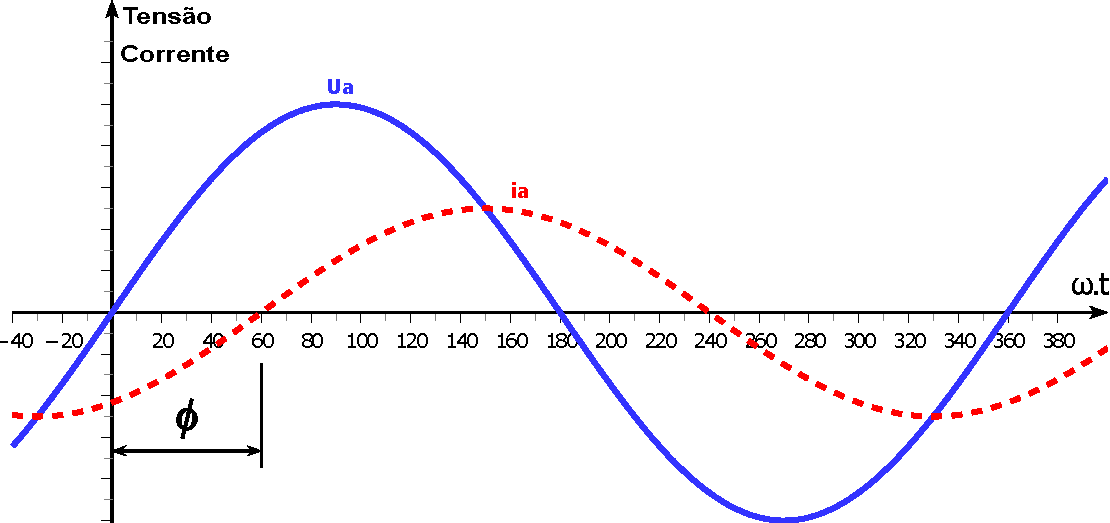
\includegraphics[width=15.3cm]{arquivos/GraficoFP.pdf}
    \FonteFig{Próprio Autor}
    \caption{Curvas de Tensão e Corrente em Carga Indutiva com Ângulo~$\phi$ de Fator de Potência}
    \label{fig:GraficoFP}
\end{figure}  

Legenda:\\
\vspace{-1.3cm}
\begin{tabbing}
    \hspace{1cm}  \= \hspace{1cm} \= \kill \\
    \gls{Ua}      \> $\Rightarrow$ \> Tensão na Fase A ~~~(\textcolor{blue}{\rule{3cm}{1mm}}); \\
    \gls{Ia}      \> $\Rightarrow$ \> Corrente na Fase A (\textcolor{red}{\hdashrule[0.1ex]{3.1cm}{1mm}{2mm}}); \\
    \gls{fi}    \> $\Rightarrow$ \> Ângulo do Fator de Potência; \\
    \gls{w}    \> $\Rightarrow$ \> Velocidade angular: $\omega=2\cdot \pi \cdot f$;    
\end{tabbing}

\begin{itemize}
    \item \verb|\rule{tamanho}{espessura}| cria uma linha com tamanho e espessura definidos. 
    \item \verb|\hdashrule[0.1ex]{tamanho}{espessura}{distancia entre os tracos}}| cria uma linha tracejada com tamanho, espessura e distância entre os traços definidos.
\end{itemize}

\begin{CaixaVerde}
    Perceba que a legenda possui o comando \verb|\gls{}| que adiciona os símbolos no Glossário. Para criar um glossário, veja a seção~\ref{sec:Glossario} na página~\pageref{sec:Glossario}.
\end{CaixaVerde}

\pagebreak
\begin{Codigo}[language=tex, 
    caption=Sintaxe para criar a legenda alinhada e com citação no Glossário, 
    label=cod:LegendaGraf]
\begin{tabbing}
  \hspace{1cm}  \=  \hspace{1cm}   \= \kill \\
  \gls{Ua}      \>  $\Rightarrow$  \> Tensao na Fase A
                    (\textcolor{blue}{\rule{3cm}{1mm}}); \\
  \gls{Ia}      \>  $\Rightarrow$  \> Corrente na Fase A
    (\textcolor{red}{\hdashrule[0.1ex]{3.1cm}{1mm}{2mm}}); \\
  \gls{fi}      \>  $\Rightarrow$  \> Angulo do Fator de
                                      Potencia;  \\   
\end{tabbing}
\end{Codigo}

%%%%%%%%%%%%%%%%%%%%%%%%%%%%%%%
%\pagebreak

\subsection{Tabelas}

Para adicionarmos tabelas no texto veja a sintaxe do código~\ref{cod:Tab} na página~\pageref{cod:Tab} e o resultado na tabela~\ref{tab:Tabela} ,  repare que a tabela deve vir centralizada no texto e com o título na parte de cima, e a fonte de onde foi retirada a tabela (comando \verb|\FonteTab{}|) deve vir na parte de baixo, e deve ser citada nas Referências. 

As tabelas devem ser enxutas, e devem conter somente as linhas de Cima, Meio e de Baixo, sendo que não se utiliza de linhas de coluna, nem linhas separadoras entre linhas.

\begin{CaixaVermelha}
    \begin{enumerate}
        \item Textos de palavras devem vir justificados a esquerda, para ficarem  alinhados a esquerda na coluna;
        \item Números devem vir justificados a direita, sendo que todos os números de uma mesma coluna devem vir com o mesmo número de casas decimais para alinhamento com {\bf vírgula debaixo de vírgula na coluna}.
    \end{enumerate}
\end{CaixaVermelha}

\begin{table}[htb]
    \centering
    \caption{Note que as palavras são alinhadas à esquerda e os números são alinhados à direita e com vírgula debaixo de vírgula}
    \begin{tabular}{lrr}
       \Linha % linha grossa
       {\bf Números} & {\bf 4 Casas} & {\bf Aleatórios} \\
       \hline % linha fina      
       Número $\pi$          &    3,1416  &    125,07  \\
       Núm. de Euler $e$     &    2,7182  &     79,00  \\
       Núm. de Ouro $\phi$   &    1,6180  &  1.975,23  \\
       Raiz: $\sqrt{2}$            &    1,4142  &      8,91  \\ 
       Raiz: $\sqrt{3}$            &    1,7320  &    543,10  \\
       \Linha % linha grossa
    \end{tabular}    
    \FonteTab{Cite aqui a fonte da tabela}
    \label{tab:Tabela}
\end{table}

Para alinhamento das células na coluna utilize a letra L minúscula (left) para alinhamento à esquerda, e utilize a letra R minúscula (right) para alinhamento à direita.


\pagebreak
Utilize o comando \verb|\Linha| para as linhas horizontais grossas e o comando \verb|\hline| para as linhas horizontais finas. 

As linhas da vertical devem ser evitadas para que a tabela fique a mais limpa possível.

\begin{Codigo}[language=tex, 
    caption=Sintaxe para adicionar Tabelas no Texto, 
    label=cod:Tab]
\begin{table}[htb]
    \centering
    \caption{Note que as palavras sao alinhadas a esquerda 
    e os numeros sao alinhados a direita e com 
    virgula debaixo de virgula}
    \begin{tabular}{lrr}
       \Linha % linha grossa
       {\bf Numeros}   & {\bf 4 Casas} & {\bf Aleatorios} \\
       \hline % linha fina
       Numero $\pi$        &    3,1416     &    125,07  \\
       Euler $e$           &    2,7182     &     79,00  \\
       Ouro $\phi$         &    1,6180     &  1.975,23  \\ 
       Raiz: $\sqrt{2}$    &    1,4142     &      8,91  \\ 
       Raiz: $\sqrt{3}$    &    1,7320     &    543,10  \\
       \Linha % linha grossa
    \end{tabular}    
    \FonteTab{Cite aqui a fonte da tabela}
    \label{tab:Tabela}
\end{table}
\end{Codigo}

Para citar as tabelas, utilizamos o comando \verb|~\ref{}| e para citar a página utilizamos o comando \verb|~\pageref{}|.

\subsubsection{Tabelas coloridas (opcional)} 

De forma opcional você poderá colorir as células das linhas da tabela, conforme mostra a tabela~\ref{tab:TabelaColorida}.

\begin{table}[htb]
    \centering
    \caption{Veja o alinhamento das palavras e números}
    % colore a partir da segunda linha de vermelho e verde
    \rowcolors{2}{red!20}{green!20}
    \begin{tabular}{lrlrr}
       \Linha % linha grossa
       \rowcolor{red!60} % colore a linha imediatamente abaixo
       \textbf{Fruta} & \textbf{Peso (kg)} & \textbf{Qualid.} & \textbf{R\$/kg}  &  \textbf{Total (R\$)}\\
       \Linha % linha grossa
       Maçã          & 1,250  & madura &  12,99  &  16,24 \\
       Banana Prata  & 2,510  & verde  &   8,99  &  22,56 \\
       Uva Niágara   & 1,860  & verde  &   7,09  &  13,19 \\
       Pera          & 2,110  & madura &  12,67  &  26,73 \\
       Kiwi          & 3,640  & verde  &  10,67  &  38,84 \\
       Manga Palmer  & 5,300  & madura &   5,98  &  31,69 \\
       \Linha % linha grossa
       \rowcolor{green!60} % colore a linha imediatamente abaixo
       \textbf{TOTAL} &       &        &         & {\bf 149,26} \\
       \Linha % linha grossa
    \end{tabular}    
    \FonteTab{Cite aqui a fonte da tabela}
    \label{tab:TabelaColorida}
\end{table}

\begin{itemize}
    \item \verb|\rowcolor{nome da cor}|: colore a linha imediatamente abaixo do comando;
    \item \verb|\rowcolors{num da linha}{nome da cor 1}{nome da cor 2}|: colore as linhas alternadas com a ``cor~1'' e ``cor~2'', a partir da linha especificada em ``num~da~linha'';
    \item \verb|{green!20}|: colore com 20\% da cor verde, aumente este valor para cores mais escuras;
\end{itemize}

\vspace{5mm}

O código~\ref{cod:Tab2} mostra como criar tabelas com linhas coloridas. Lembrando que colorir linhas é opcional.

\pagebreak

\begin{Codigo}[language=tex, 
    caption=Sintaxe para adicionar Tabelas Coloridas no Texto, 
    label=cod:Tab2]
\begin{table}[htb]
  \centering
  \caption{Veja o alinhamento das palavras e numeros}
  % colore a partir da segunda linha de vermelho e verde
  \rowcolors{2}{red!20}{green!20}
  \begin{tabular}{lrlrr}
    \Linha % linha grossa
    \rowcolor{red!60} % colore a linha imediatamente abaixo
    \textbf{Fruta} & \textbf{Peso (kg)} & \textbf{Qualid.} &
    \textbf{R\$/kg}  &  \textbf{Total (R\$)}\\
    \Linha % linha grossa
    Maca          & 1,250  & madura &  12,99  &  16,24 \\
    Banana Prata  & 2,510  & verde  &   8,99  &  22,56 \\
    Uva Niagara   & 1,860  & verde  &   7,09  &  13,19 \\
    Pera          & 2,110  & madura &  12,67  &  26,73 \\
    Kiwi          & 3,640  & verde  &  10,67  &  38,84 \\
    Manga Palmer  & 5,300  & madura &   5,98  &  31,69 \\
    \Linha % linha grossa
    \rowcolor{green!60} % colore a linha imediatamente abaixo
    \textbf{TOTAL} &    &     &      & {\bf 149,26} \\
    \Linha % linha grossa
  \end{tabular}    
  \FonteTab{Cite aqui a fonte da tabela}
  \label{tab:TabelaColorida}
\end{table}

\end{Codigo}

%%%%%%%%%%%%%%%%%%%%%%%%%%%%%%%
\pagebreak\clearpage\newpage

\subsection{Equações}

Para adicionar equações no texto, utiliza-se a sintaxe normal do ~\LaTeX, o comando \verb|\begin{equation}|, conforme mostra a equação~\ref{eq:NumEsp}, lembrando que os símbolos devem possuir legenda próxima à equação, e devem ser adicionadas também no glossário:

\begin{equation}
    N_1 = \frac{\sqrt{2}}{2 \cdot \pi } \cdot \frac{U_1 \cdot  10^8}{f \cdot S_L \cdot B} \quad \Rightarrow \quad N_1 = \frac{U_1 \cdot 10^8}{4,44 \cdot f \cdot S_L \cdot B}
    \label{eq:NumEsp}
\end{equation}

Sendo que:\\
\vspace{-1.5cm}
\begin{tabbing}
    \hspace{1cm}  \= \hspace{1cm} \= \kill \\
    \gls{N1}      \> $\Rightarrow$ \> Número de espiras do primário; \\
    \gls{U1}      \> $\Rightarrow$ \> Tensão do primário (V); \\
    \gls{freq}    \> $\Rightarrow$ \> frequência (Hz); \\
    \gls{SL}      \> $\Rightarrow$ \> Área da Seção Líquida do núcleo ($cm^2$); \\
    \gls{DenFlux} \> $\Rightarrow$ \> Densidade de Fluxo Magnético (G = Gauss); 
\end{tabbing}

\vspace{4mm}
\begin{CaixaVermelha}
    Todas as equações precisam ser numeradas e citadas ao longo do texto, bem como devem possuir a legenda dos símbolos (abaixo da equação) quando a equação aparece pela primeira vez no texto.
\end{CaixaVermelha}

%\pagebreak\newpage\clearpage

O código para gerar a equação~\ref{eq:NumEsp} da página~\pageref{eq:NumEsp} segue no código~\ref{cod:EqNumEsp}:

\begin{Codigo}[language=tex, 
    caption=Sintaxe para adicionar Equações, 
    label=cod:EqNumEsp]
\begin{equation}
   N_1=\frac{\sqrt{2}}{2 \cdot \pi } \cdot
   \frac{U_1 \cdot  10^8}{f \cdot S_L \cdot B}
   \quad \Rightarrow \quad 
   N_1=\frac{U_1 \cdot 10^8}{4,44 \cdot f \cdot S_L \cdot B}
   \label{eq:NumEsp}
\end{equation}
\end{Codigo}

A sintaxe do código para gerar a legenda está descrita no código . Perceba que o comando \verb|\gls{}| envia o símbolo para o Glossário. Para criar um glossário, veja a seção~\ref{sec:Glossario} na página~\pageref{sec:Glossario}.

\begin{Codigo}[language=tex, 
    caption=Sintaxe para adicionar Legendas alinhadas e com citações no Glossário, 
    label=cod:LegendaNumEsp]
Sendo que:\\
\begin{tabbing}
  \hspace{1cm}  \= \hspace{1cm} \= \kill \\
  \gls{N1}      \> $\Rightarrow$ \> Numero de espiras do 
                                    primario; \\
  \gls{U1}      \> $\Rightarrow$ \> Tensao do primario(V);\\
  \gls{freq}    \> $\Rightarrow$ \> frequencia (Hz); \\
  \gls{SL}      \> $\Rightarrow$ \> Area da Secao Liquida 
                                    do nucleo ($cm^2$); \\
  \gls{DenFlux} \> $\Rightarrow$ \> Densidade de Fluxo 
                                    Magnetico (G = Gauss); 
\end{tabbing}
\end{Codigo}

Segue um exemplo do comando \verb|\begin{eqnarray}| para {\bf alinhar resoluções matemáticas}, citando a equação da primeira linha~\ref{eq:EqL1}, a equação da segunda linha~\ref{eq:EqL2} e a equação da terceira linha~\ref{eq:EqL3}:

\begin{eqnarray}
    \label{eq:EqL1}
    10x^2y+15xy^2-5xy & = & 5(2x^2y+3xy^2-xy) \\    
    \label{eq:EqL2}
                      & = & 5x(2xy+3y^2-y) \\
    \label{eq:EqL3}
                      & = & 5xy(2x+3y-1)    
\end{eqnarray}

\begin{Codigo}[language=tex, 
    caption=Comando eqnarray com todas as equações numeradas, 
    label=cod:Eqnarray]
  \begin{eqnarray}
    \label{eq:EqL1}
    10x^2y+15xy^2-5xy & = & 5(2x^2y+3xy^2-xy) \\    
    \label{eq:EqL2}
                      & = & 5x(2xy+3y^2-y) \\
    \label{eq:EqL3}
                      & = & 5xy(2x+3y-1)    
  \end{eqnarray}
\end{Codigo}

Caso queiramos numerar apenas algumas linhas do comando \verb|\begin{eqnarray}|, basta inserir o comando \verb|\nonumber| nas linhas que não serão numeradas, veja a equação~\ref{eq:EqL4}:
%
\begin{eqnarray}
    10x^2y+15xy^2-5xy   & = & 5(2x^2y+3xy^2-xy) \nonumber \\
                        & = & 5x(2xy+3y^2-y)    \nonumber \\
    \label{eq:EqL4}
                        & = & 5xy(2x+3y-1)
\end{eqnarray}

\begin{Codigo}[language=tex, 
    caption=Comando eqnarray com somente uma equação numerada, 
    label=cod:EqnarrayNonumber]
  \begin{eqnarray}
    10x^2y+15xy^2-5xy   & = & 5(2x^2y+3xy^2-xy) \nonumber \\
                        & = & 5x(2xy+3y^2-y)    \nonumber \\
    \label{eq:EqL4}
                        & = & 5xy(2x+3y-1)
  \end{eqnarray}
\end{Codigo}

%%%%%%%%%%%%%%%%%%%%%%%%%%%%%%%%%%%%


\subsection{Caixas Coloridas}

A classe \verb|cls-PFC-COEEL.cls| possui algumas caixas coloridas padronizadas na cor verde e na cor vermelha, conforme mostra o código~\ref{cod:Caixas}.

\vspace{5mm}
\begin{CaixaVerde}
    Exemplo de uma caixa verde com marcação inferior na cor RGB verde (50,160,65) padrão dos Institutos Federais.
\end{CaixaVerde}

\vspace{5mm}
\begin{CaixaVermelha}
    Exemplo de uma caixa vermelha com marcação esquerda na cor RGB vermelha (200,25,30) padrão dos Institutos Federais.
\end{CaixaVermelha}

\clearpage\newpage\pagebreak

\begin{Codigo}[language=tex, 
    caption=Sintaxe para adicionar Caixas Coloridas no Texto, 
    label=cod:Caixas]
    % para criar uma caixa verde
    \begin{CaixaVerde}
        Exemplo de uma caixa verde com marcacao inferior 
        na cor RGB verde (50,160,65) padrao dos Institutos 
        Federais.
    \end{CaixaVerde}
    
    % para criar uma caixa vermelha
    \begin{CaixaVermelha}
        Exemplo de uma caixa vermelha com marcacao esquerda 
        na cor RGB vermelha (200,25,30) padrao dos Institutos 
        Federais.
    \end{CaixaVermelha}
\end{Codigo}



\vspace{1cm}
Caso você queira utilizar diferentes caixas coloridas além destas duas padronizadas, procure pelo pacote {\bf tcolorbox}. Um ótimo exemplo pode ser encontrado em:

\hspace{-1.2cm}{\footnotesize\url{ https://www.overleaf.com/latex/examples/drawing-coloured-boxes-using-tcolorbox/pvknncpjyfbp}}

%%%%%%%%%%%%%%%%%%%%%%%%%%%%%
\clearpage\newpage\pagebreak

\section{Capítulos, Seções, Subseções, Subsubseções, Parágrafos e Subparágrafos}

A classe \verb|cls-PDC-COEEL.cls| está configurada para a numeração dos
Capítulos Seções, Subseções, Subsubseções, Parágrafos e Subparágrafos:

\begin{itemize}
    \item \verb|\chapter{}| = Capítulo: Capítulo 1;
    \item \verb|\section{}| = Seção: Numeração do capítulo seguido do número da seção: 1.1;
    \item \verb|\subsection{}| = Subseção: Numeração do capítulo seguido do número da seção e da subseção: 1.1.1;
    \item \verb|\subsubsection{}| = Subsubseção: Numeração do capítulo seguido do número da seção, subseção e subsubseção: 1.1.1.1;
    \item \verb|\paragraph{}| = Parágrafo: Numeração dos parágrafos em letras alfabéticas seguidas de parênteses: a);
    \item \verb|\subparagraph{}| = Subparágrafos: Numeração dos subparágrafos em números romanos minúsculos seguidos de parênteses: i)
\end{itemize}

\subsection{Exemplo de Subseção}
Este é o exemplo de uma subseção\ldots

\subsubsection{Exemplo de uma Subsubseção}
Este é o exemplo de uma subsubseção\ldots

\paragraph{Exemplo de um Parágrafo}
Este é o exemplo de um parágrafo\ldots

\subparagraph{Exemplo de um Subparágrafo}
Este é o exemplo de um subparágrafo\ldots


%%%%%%%%%%%%%%%%%%%%%%%%%%%%%%

\subsection{Utilizando o BibTeX}
\label{sec:BibTeX}

Para este template de PFC e Relatório, foi criada uma biblioteca exemplo com o nome {\bf BIB\_pfc.bib}, que você pode encontrar na figura~\ref{fig:bib_pfc}. 

Veja na figura~\ref{fig:bib_pfc} o formato do código \LaTeX~ do arquivo {\bf BIB\_pfc.bib}.

\begin{figure}[htb]
    \centering  
    \FonteFig{Próprio Autor}
    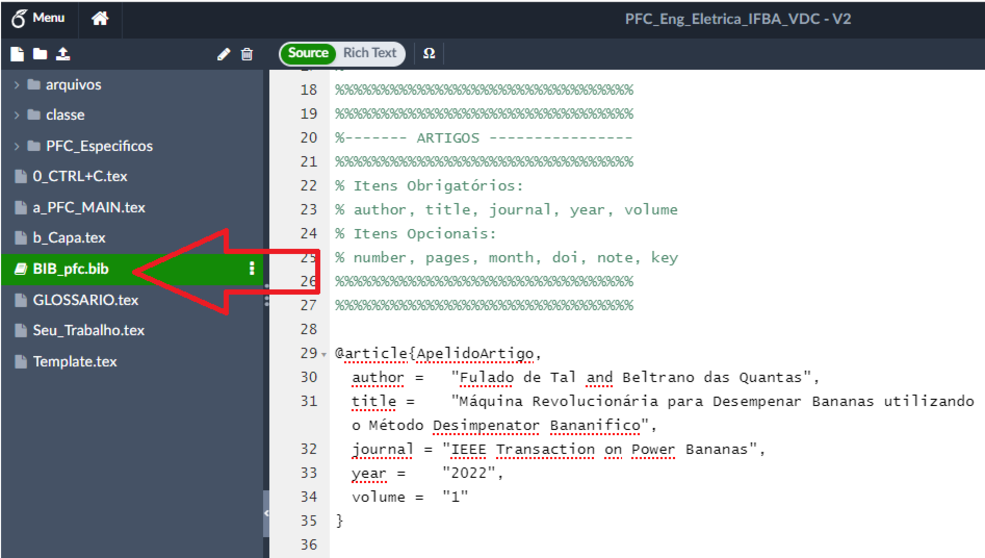
\includegraphics[width=15cm]{classe/arqcls/Fig_bib_pfc.pdf}
    \caption{Localização da biblioteca  {\bf BIB\_pfc.bib} criada para este template no LaTeX-Overleaf}    
    \label{fig:bib_pfc}
\end{figure}

\vspace{6mm}
\begin{CaixaVerde}
    Acrescente todas as suas referências a serem utilizadas no seu trabalho aqui neste arquivo {\bf BIB\_pfc.bib}
\end{CaixaVerde}

\vspace{6mm}
Um exemplo de formatação de citação do artigo~\cite{ApelidoArtigo}, também pode ser citado com o nome do autor desta forma~\citeonline{ApelidoArtigo}. Esta citação no arquivo {\bf BIB\_pfc.bib} está mostrado no código~\ref{cod:BibTeX}.  

\pagebreak
\begin{Codigo}[language=tex, 
    caption=Exemplo de alimentação do arquivo {BIB\_pfc.bib}, 
    label=cod:BibTeX]
  @article{ApelidoArtigo,
  author =   "Fulado de Tal and Beltrano das Quantas",
  title =    "Maquina Revolucionaria para Desempenar Bananas 
              Utilizando o Metodo Desimpenator Bananifico",
  journal = "IEEE Transaction on Power Bananas", 
  year =    "2022",
  volume =  "1"
}
\end{Codigo}


No arquivo {\bf BIB\_pfc.bib} estão as orientações de como acrescentar suas referências, contendo os itens obrigatórios e opcionais. As referências suportadas mais utilizadas são mostradas na tabela~\ref{tab:Tipos_Ref}: 
    
\begin{table}[htb]
    \centering
    \caption{Principais tipos de referências mais utilizadas}
    \begin{tabular}{ll}
        \toprule
        Article         & = Artigos \\
        Book            & = Livros \\
        Manual          & = Manuais \\
        mastersthesis   & = Dissertações de Mestrado \\
        phdthesis       & = Teses de Doutorado \\
        techreport      & = Normas Técnicas \\
        unpublished     & = Citações da Internet\\
        \bottomrule
    \end{tabular}        
    \label{tab:Tipos_Ref}
\end{table}
    
 Para  mais tipos de referências além das citadas na tabela~\ref{tab:Tipos_Ref}, consulte o site da ferramenta BibTeX: \url{https://en.wikipedia.org/wiki/BibTeX}. 
Aqui neste modelo (template) está configurado a ferramenta {\bf AbnTeX2Cite} \cite{AbnTeX2Cite} que segue a norma brasileira ~\citeonline{NBR6023_Referencias}.

%%%%%%%%%%%%%%%%%%%%%%%%%%%%

\subsection{Citações de Referências com os comandos: cite e  citeonline}

Os comandos de citação mais utilizados são: \verb|\cite{}| e  \verb|\citeonline{}|. Existem outros formatos específicos que podem ser consultados no manual da ferramenta {\bf AbnTex2Cite} \cite{AbnTeX2Cite}.

Note que após realizar a citação no texto o ~\LaTeX~ já cria automaticamente as referências no capítulo de referências formatado de acordo com a norma~\citeonline{NBR6023_Referencias}, conforme mostrado no capítulo de Referências na página~\pageref{cap:RefBib}.


O comando \verb|\cite{}| cita a referência no texto da seguinte forma: \cite{ApelidoArtigo}, já o comando \verb|\citeonline{}| cita uma referência chamando o autor no texto como por exemplo: "De acordo com \citeonline{ApelidoArtigo} as poderosas máquinas de desempenar bananas\ldots"

 Para mais detalhes de como utilizar a ferramenta de citações automáticas e se precisar de mais comandos específicos para citações, de acordo com a \citeonline{NBR6023_Referencias}, consulte o documento {\bf AbnTex2Cite}:

 \url{http://tug.ctan.org/macros/latex/contrib/abntex2/doc/abntex2cite.pdf}


\section{Realizar as Referências buscando em repositórios e bases de dados indexados}

As referências devem ser citadas ao longo do texto e devem conter livros, normas, manuais e artigos que foram utilizados como literatura para o projeto.
    
Evitar referências a apostilas e sites de internet com conteúdo não revisado, como blogs e wikipedia, pois como não estão sujeitos a revisão, podem conter conteúdo errado ou não regulamentado.

Para que a referência que você irá citar tenha relevância, ela precisa ter vindo de alguma fonte que foi revisada por profissionais especializados na área. Os livros, dissertações de mestrado, teses de doutorado, artigos de revistas e conferências científicas, passam por correções e avaliações por pares, validando o conteúdo científico.  
    
Procure selecionar sites de internet que são confiáveis e revisados, tais como sites de:

\begin{enumerate}
    \item Revistas científicas indexadas;
    \item Conferências e congressos;
    \item Teses, Dissertações, Monografias;
    \item Patentes;
    \item Repositórios Científicos;
    \item Fabricantes;
    \item Manuais de utilização;
    \item Normas Técnicas (ABNT, IEEE, IEC, ISO\ldots);
    \item Normas Regulamentadoras (NR);  
    \item Legislação;
    \item Universidades;
\end{enumerate}

Seguem alguns exemplos de fontes confiáveis:

\begin{itemize}
    \item Domínio Público do MEC:\\
    \url{http://www.dominiopublico.gov.br/};

    \item Periódicos da Capes:\\
    \url{http://www.periodicos.capes.gov.br/} ;

    \item Periódicos Compendex:\\
    \url{https://www.engineeringvillage.com/search/quick.url}

    \item Espacenet: \\ \url{http://worldwide.espacenet.com/}

    \item IEEE Xplore: \\
    \url{http://ieeexplore.ieee.org/Xplore/home.jsp}%

    \item Science Direct: \\
    \url{https://www.sciencedirect.com/}
    
    \item SciELO - Brasil: \\
    \url{https://www.scielo.br/}

    \item Google Acadêmico: \\
    \url{https://scholar.google.com.br/?hl=pt}

    \item Elsevier: \\
    \url{https://www.elsevier.com/pt-br}
\end{itemize}

Outra forma confiável é a busca em  repositórios de Teses e Dissertações de Universidades.

Um ótimo vídeo sobre como realizar busca nas bases {\bf Science Direct} pode ser encontrado no canal ~"Descomplicando"~ do professor Henrique R. Frigeri: \url{https://youtu.be/ThcB65kcuiM}.

%%%%%%%%%%%%%%%%%%%%%%%%%%%%

\section{Organizador de Referências: Mendeley}

Mendeley é uma empresa sediada em Londres, Reino Unido, que desenvolve produtos e serviços para pesquisadores acadêmicos. É conhecida principalmente por seu {\bf gerenciador de referências, usado para gerenciar, compartilhar e criar referências bibliográficas para artigos acadêmicos}.

O Mendeley pode ser acessado em \url{https://www.mendeley.com/}, e pode ser utilizado em sua forma online ou pode ser feito o download do programa de gerenciamento de referências.

Mendeley é um gerenciador de referências e uma rede social acadêmica que ajuda a organizar sua pesquisa, colaborar com outras pessoas on-line e descobrir as pesquisas mais recentes.

\begin{CaixaVerde}
    O Mendeley fornece um {\bf gerenciador de referência gratuito} que auxilia nos trabalhos acadêmicos e tem a finalidade de gerenciar arquivos eletrônicos (formato PDF), além de ajudar na normalização de citações e referências geradas automaticamente.
\end{CaixaVerde}

\begin{CaixaVermelha}
    {\large O Mendeley gera automaticamente referências no formato {\bf BibTeX}.}
\end{CaixaVermelha}

Você pode criar uma conta gratuita e acessar sua biblioteca em qualquer lugar. Além disso, você pode gerar referências, citações e bibliografias em uma ampla variedade de estilos de revistas com apenas alguns cliques. Você também pode ler artigos em qualquer lugar com aplicativos para iOS e Android.

Um ótimo vídeo sobre o Mendeley pode ser acessado no canal do professor Lucas Pantuza Amorim: \url{https://youtu.be/rCQhAJlW4qc}.

%%%%%%%%%%%%%%%%%%%%%%

\subsection{Vantagens em utilizar o gerenciador de referências Mendeley}

Algumas vantagens em utilizar o Mendeley para gerenciar as referências de sua pesquisa:

\begin{itemize}
    \item Ajuda a organizar sua pesquisa e gerenciar arquivos eletrônicos (formato PDF);
    \item Ajuda na normalização de citações e referências geradas automaticamente;
    \item Permite acessar sua biblioteca em qualquer lugar;
    \item Permite gerar referências, citações e bibliografias em uma ampla variedade de estilos de revistas com apenas alguns cliques;
    \item {\bf Exporta referências no formato BibTeX};
    \item É uma rede social acadêmica que permite colaborar com outras pessoas on-line e descobrir as pesquisas mais recentes;
    \item Possui aplicativos para iOS e Android para ler artigos em qualquer lugar;
    \item O Mendeley organiza todos os seus artigos, documentos, etc, ajuda a localizar o texto que você precisa, e exporta a referência no formato que você precisar (BibTeX por exemplo);
    \item Ao invés de você guardar todos as suas dezenas de  artigos e referências em uma pasta no computador e depois não saber mais qual deles tem o texto que você precisa, você irá guardar tudo no Mendeley e quando precisar, o Mendeley te ajudará a encontrar o que precisar.
    \item Com o Mendeley você poderá fazer anotações, grifar, registrar e comentar suas referências de forma a conseguir encontrar o que precisa na hora de escrever seu trabalho definitivo;
    \item O Mendeley te ajuda a criar o capítulo de Referencial Teórico com levantamento bibliográfico;
\end{itemize}

\begin{CaixaVerde}
    Imagine que você já leu dezenas de artigos, manuais, documentos, teses e dissertações no tema de seu projeto, porém na hora de escrever o capítulo de Referencial Teórico {\bf você não lembra mais} qual foi o artigo que está um determinado assunto que você precisa citar. {\bf Pode ter certeza que isso vai acontecer,} e o Mendeley foi feito para organizar suas referências para que você consiga encontrar tudo o que precisa.
\end{CaixaVerde}

